
\preClass{Complex Numbers}

\begin{problem}
\item Plot and then convert each point in the complex plane into polar
  coordinates. Label the radius and angle in each case.

  \begin{subproblem}
  \item $3+7i$

      \iftoggle{solutions}{%

        \begin{eqnarray*}
          r & = & \sqrt{3^2 + 7^2}, \\
            & = & \sqrt{58}, \\
          \tan(\theta) & = & \frac{7}{3}, \\
          \theta & \approx & 1.166
        \end{eqnarray*}
        
        \centerline{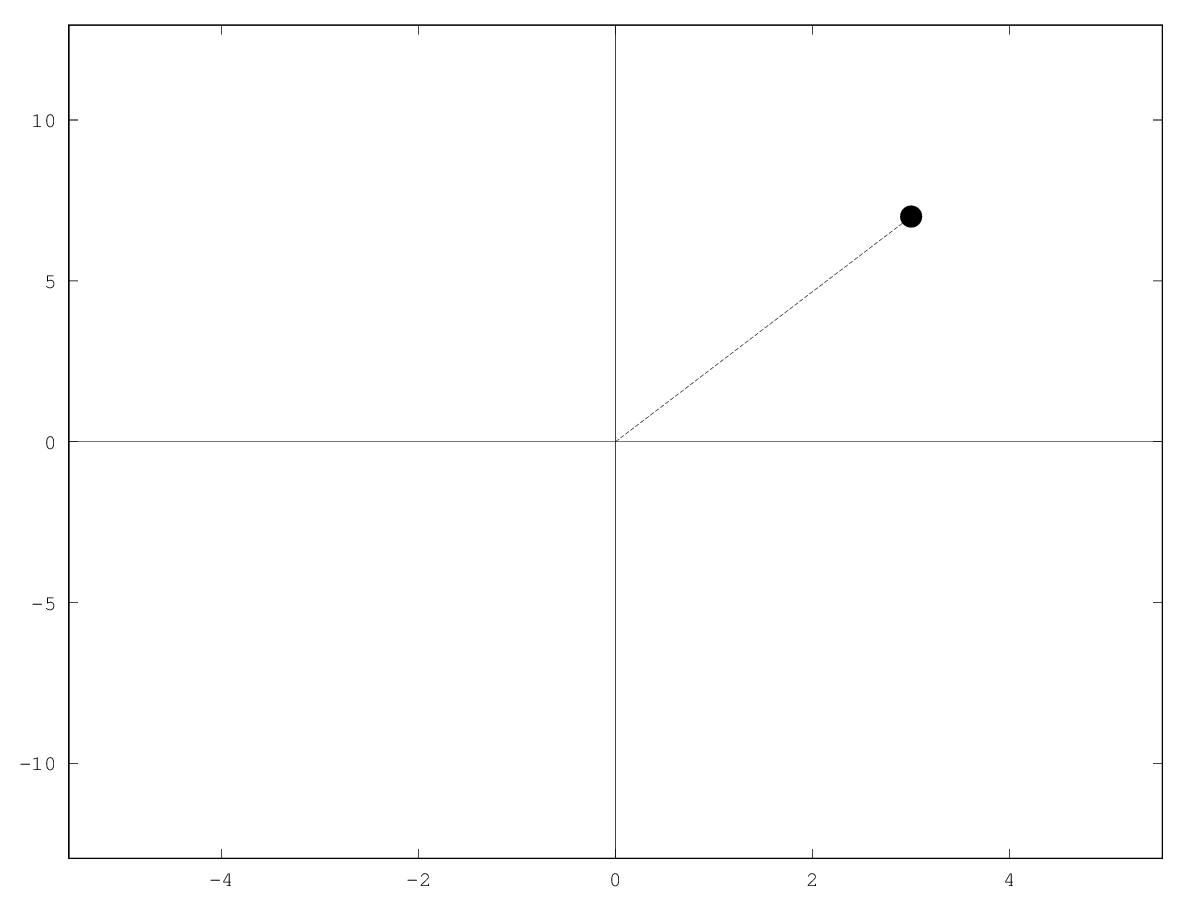
\includegraphics[width=5cm]{img/complexNumber+3+7i}}
      }

    \vfill

  \item $-3+7i$

      \iftoggle{solutions}{%

        \begin{eqnarray*}
          r & = & \sqrt{3^2 + 7^2}, \\
            & = & \sqrt{58}, \\
          \tan(\theta) & = & \frac{7}{-3}, \\
          \theta & \approx & 1.98
        \end{eqnarray*}
        
        \centerline{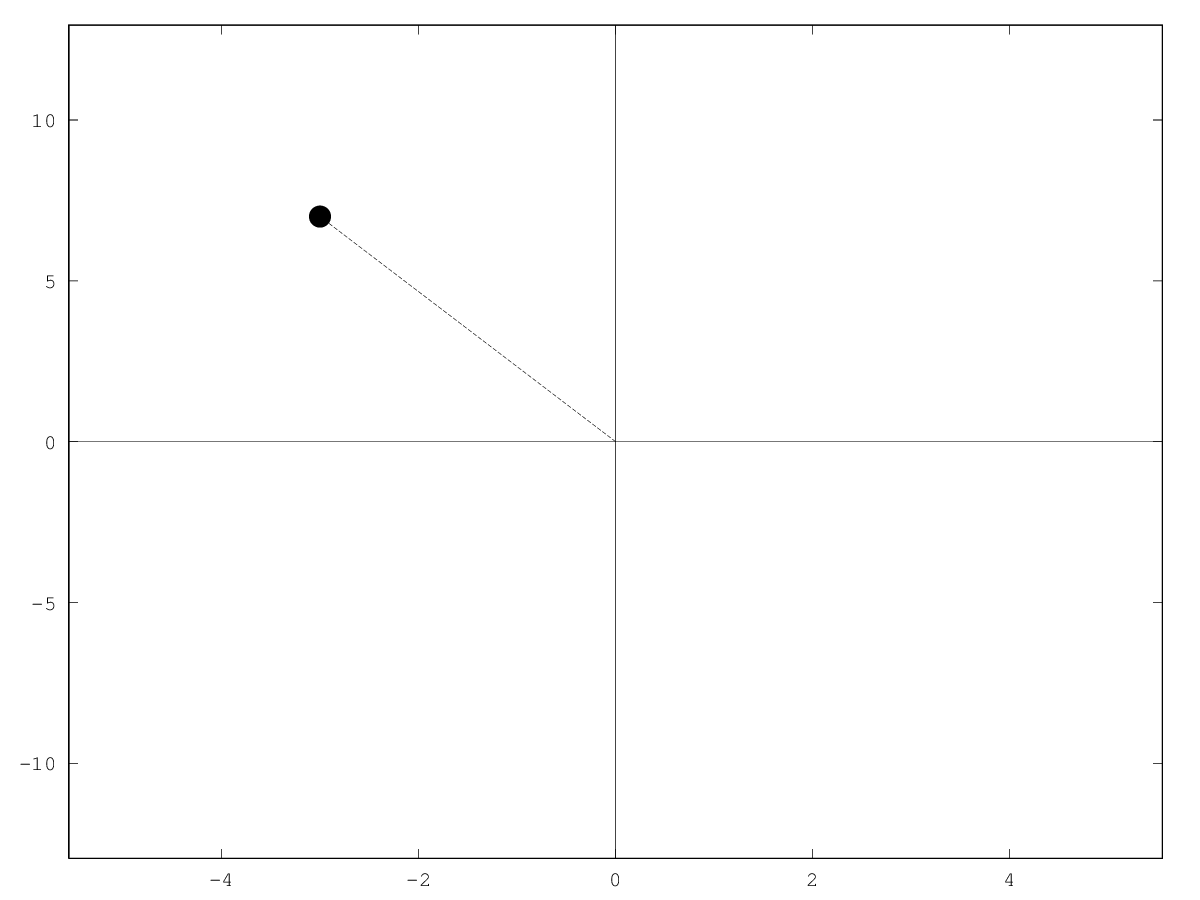
\includegraphics[width=5cm]{img/complexNumber-3+7i}}
        
      }

    \vfill

    (See the next page.)
    \clearpage

  \item $-4+2i$

      \iftoggle{solutions}{%

        \begin{eqnarray*}
          r & = & \sqrt{(-4)^2+2^2}, \\
            & = & \sqrt{20}, \\
          \tan(\theta) & = & \frac{2}{-4}, \\
          \theta & \approx & 2.18
        \end{eqnarray*}
        
        \centerline{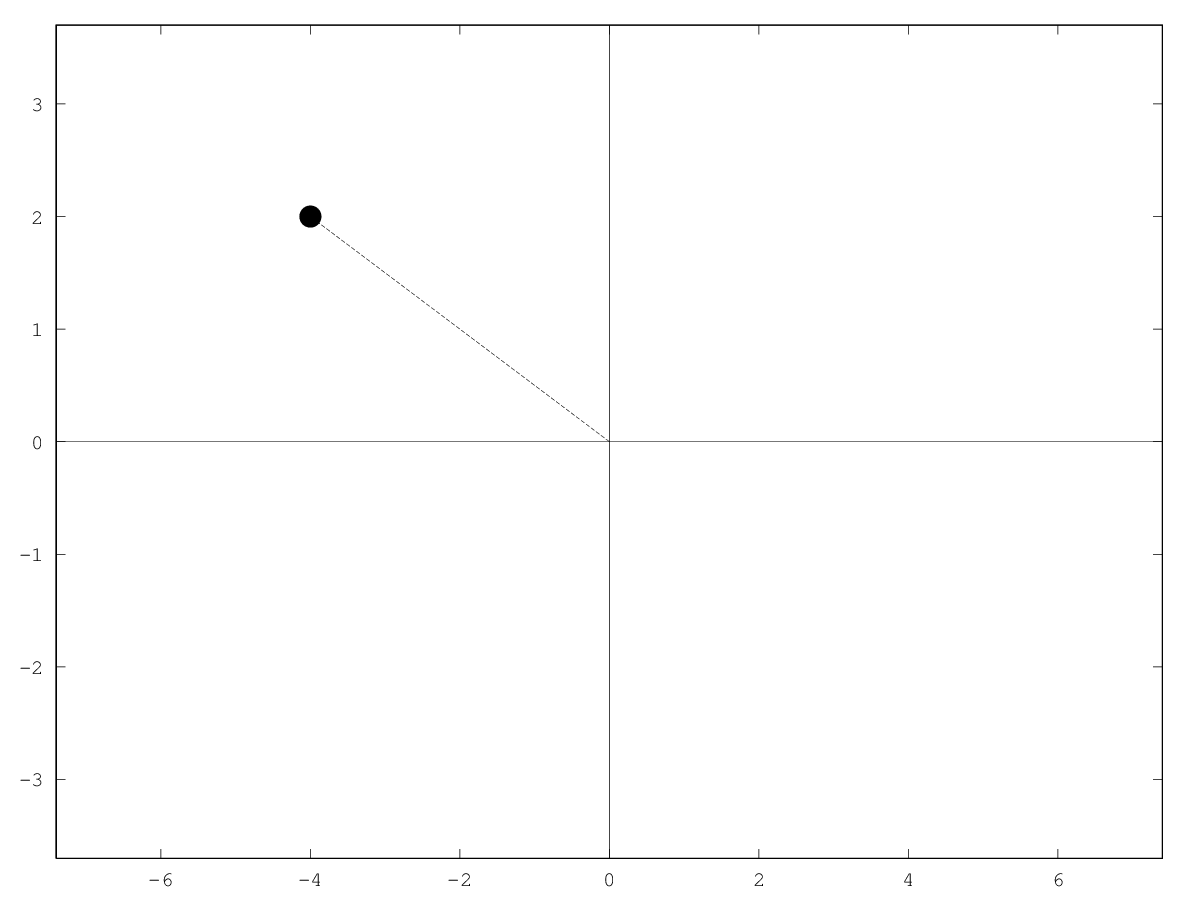
\includegraphics[width=5cm]{img/complexNumber-4+2i}}
        
      }

    \vfill

  \item $3-1i$

      \iftoggle{solutions}{%

        \begin{eqnarray*}
          r & = & \sqrt{3^2+(-1)^2}, \\
            & = & \sqrt{10}, \\
          \tan(\theta) & = & \frac{-1}{3}, \\
          \theta & \approx & -.322
        \end{eqnarray*}
        
        \centerline{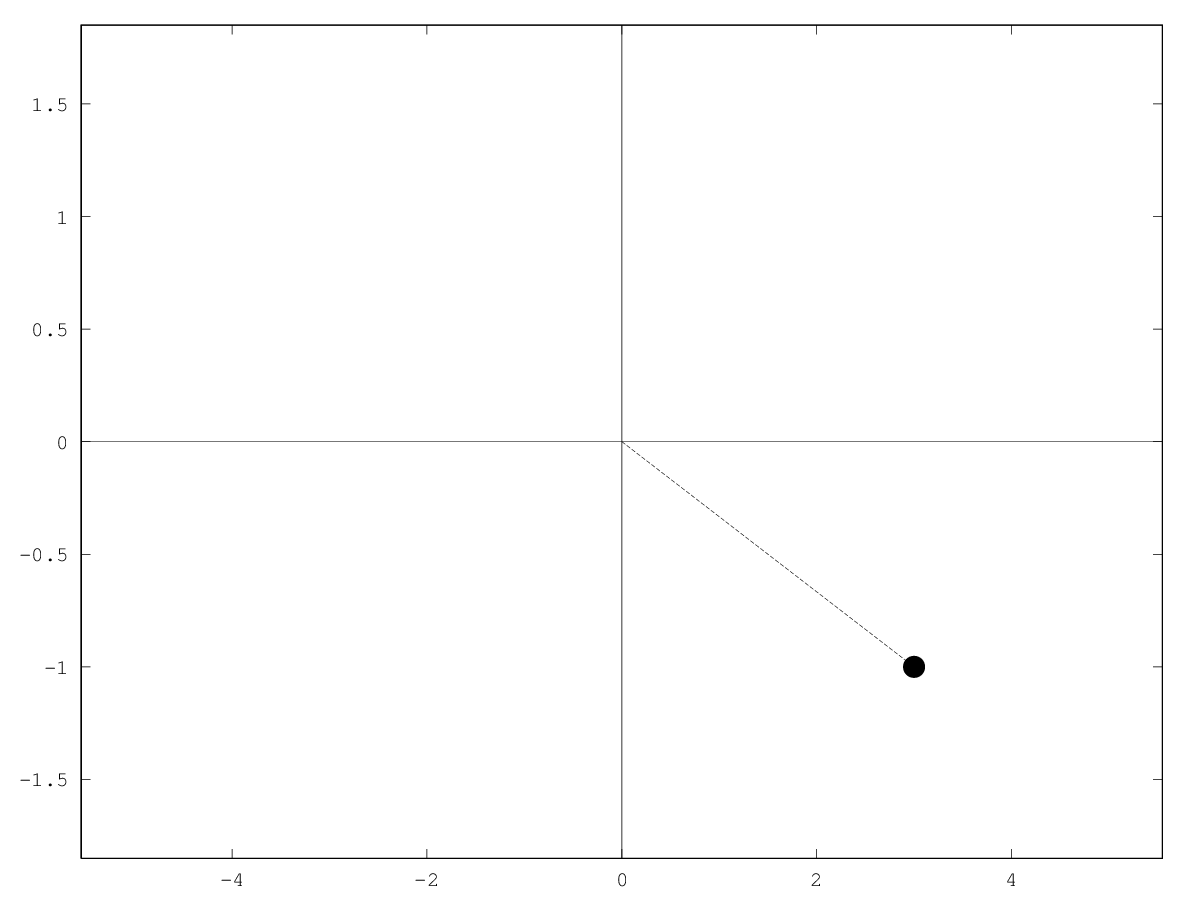
\includegraphics[width=5cm]{img/complexNumber+3-i}}

      }

    \vfill

  \end{subproblem}
\end{problem}


  \actTitle{Complex Numbers}
  \begin{problem}
  \item Expand and simplify the following expressions:
    \begin{subproblem}
      \item $(1+i)(3-i)$

      \iftoggle{solutions}{%

        \begin{eqnarray*}
          (1+i)(3-i)& = & 3 + 3i - i + 1, \\
          & = & 4 + 2i.
        \end{eqnarray*}
        
      }

        \vfill

      \item $(3+2i)(1-i)(7+2i)$

      \iftoggle{solutions}{%

        \begin{eqnarray*}
          (3+2i)(1-i)(7+2i) & = & (3 + 2i - 3i + 2)(7+2i), \\
          & = & (5-i)(7+2i), \\
          & = & 35 + 10i - 7i + 2, \\
          & = & 37 + 3i.
        \end{eqnarray*}
        
      }

        \vfill

      \item $\frac{1+2i}{4+7i}$

      \iftoggle{solutions}{%

        \begin{eqnarray*}
          \frac{1+2i}{4+7i} & = &
          \frac{1+2i}{4+7i}\cdot\frac{4-7i}{4-7i}, \\
          & = & \frac{18 + 15 i}{65}, \\
          & = & \frac{18}{65} + \frac{15}{65} i.
        \end{eqnarray*}
        
      }

        \vfill

      \item $\frac{\overline{4-i}}{3-i}(2+i)$

      \iftoggle{solutions}{%

        \begin{eqnarray*}
          \frac{\overline{4-i}}{3-i}(2+i) & = & \frac{(4+i)(2+i)}{3-i}, \\
          & = & \frac{7+6i}{3-i}, \\
          & = & \frac{7+6i}{3-i}\cdot\frac{3+i}{3+i}, \\
          & = & \frac{15 + 25i}{10}, \\
          & = & \frac{3}{2} + \frac{5}{2}i.
        \end{eqnarray*}
        
      }

        \vfill

    \end{subproblem}

    \clearpage

  \item Express each of the following numbers in the form $a+bi$:
    \begin{subproblem}
    \item $e^{i\pi/4}$

      \iftoggle{solutions}{%

        \begin{eqnarray*}
          e^{i\pi/4} & = & \cos\lp\frac{\pi}{4}\rp + i \sin\lp\frac{\pi}{4}\rp, \\
          & = & \frac{\sqrt{2}}{2} + i \frac{\sqrt{2}}{2}.
        \end{eqnarray*}
        
      }

      \vfill
    \item $2e^{i 3\pi/2}$

      \iftoggle{solutions}{%

        \begin{eqnarray*}
          2e^{i 3\pi/2} & = & 2 \cos\lp\frac{3\pi}{2}\rp + 2\sin\lp\frac{3\pi}{2}\rp, \\
          & = & -2i.
        \end{eqnarray*}
        
      }

      \vfill
    \item $10e^{i \pi/3}$

      \iftoggle{solutions}{%

        \begin{eqnarray*}
          10e^{i \pi/3} & = & 10 \cos\lp\frac{\pi}{3}\rp + i 10 \sin\lp\frac{\pi}{3}\rp, \\
          & = & 5  + i 5\sqrt{3}.
        \end{eqnarray*}
        
      }

      \vfill
    \item $4e^{i \pi}$

      \iftoggle{solutions}{%

        \begin{eqnarray*}
          4e^{i \pi} & = & 4 \cos\lp\pi\rp + i 4 \sin\lp\pi\rp, \\
          &  = & -4.
        \end{eqnarray*}
        
      }

      \vfill
    \end{subproblem}


  \end{problem}


  \actTitle{Complex Numbers}
  \begin{problem}

  \item Plot each of the following numbers in the complex plane and
    then express them in Euler form:
    \begin{subproblem}
      \item $1+i$

      \iftoggle{solutions}{%

        \begin{eqnarray*}
          r & = & \sqrt{1^2 + 1^2}, \\
            & = & \sqrt{2}, \\
          \tan(\theta) & = & \frac{1}{1}, \\
          \theta & = & \frac{\pi}{4}, \\
          z & = & \sqrt{2}e^{i\frac{\pi}{4}}.
        \end{eqnarray*}
        
        \centerline{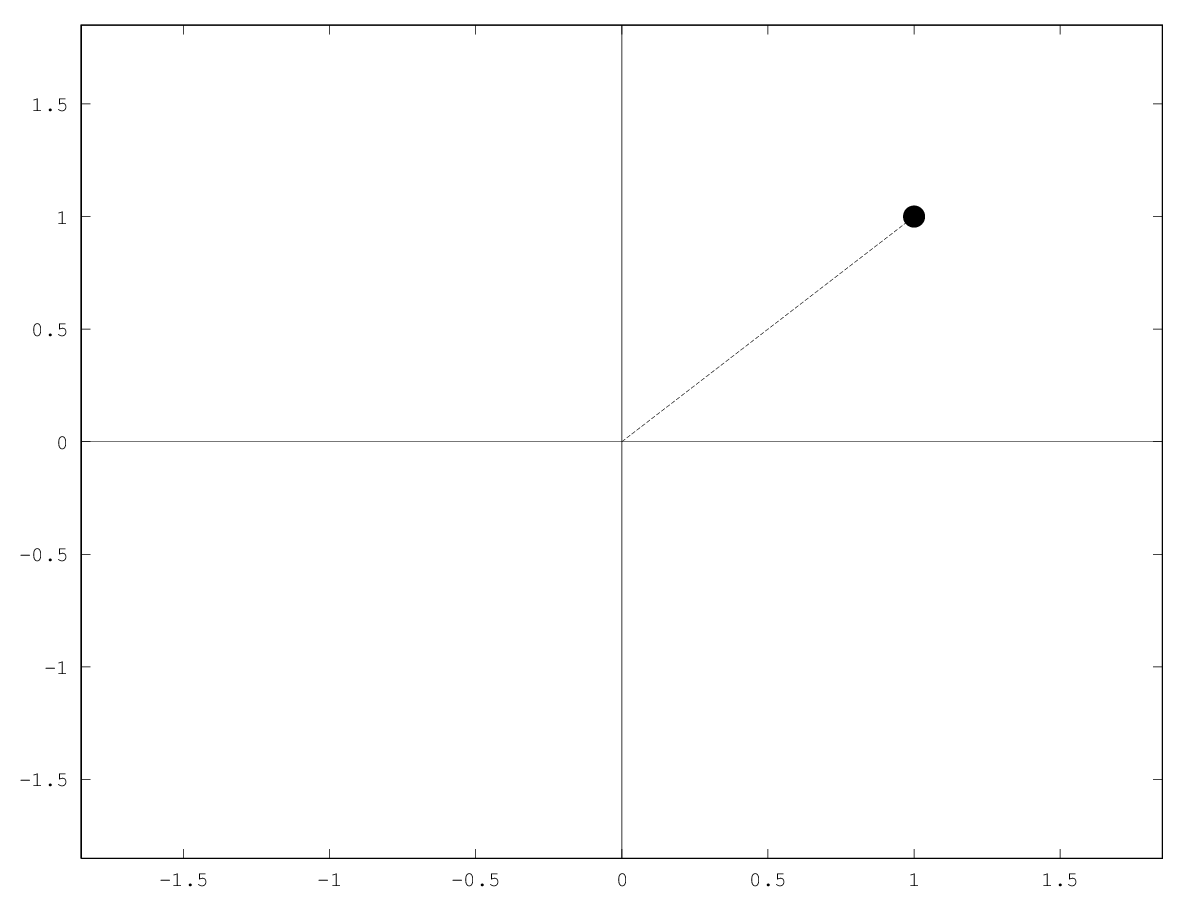
\includegraphics[width=4cm]{img/complexNumber+1+i}}
        
      }

        \vfill
      \item $1-i$

      \iftoggle{solutions}{%

        \begin{eqnarray*}
          r & = & \sqrt{1^2 + (-1)^2}, \\
            & = & \sqrt{2}, \\
          \tan(\theta) & = & \frac{-1}{1}, \\
          \theta & = & \frac{-\pi}{4}, \\
          z & = & \sqrt{2}e^{i\frac{-\pi}{4}}.
        \end{eqnarray*}
        
        \centerline{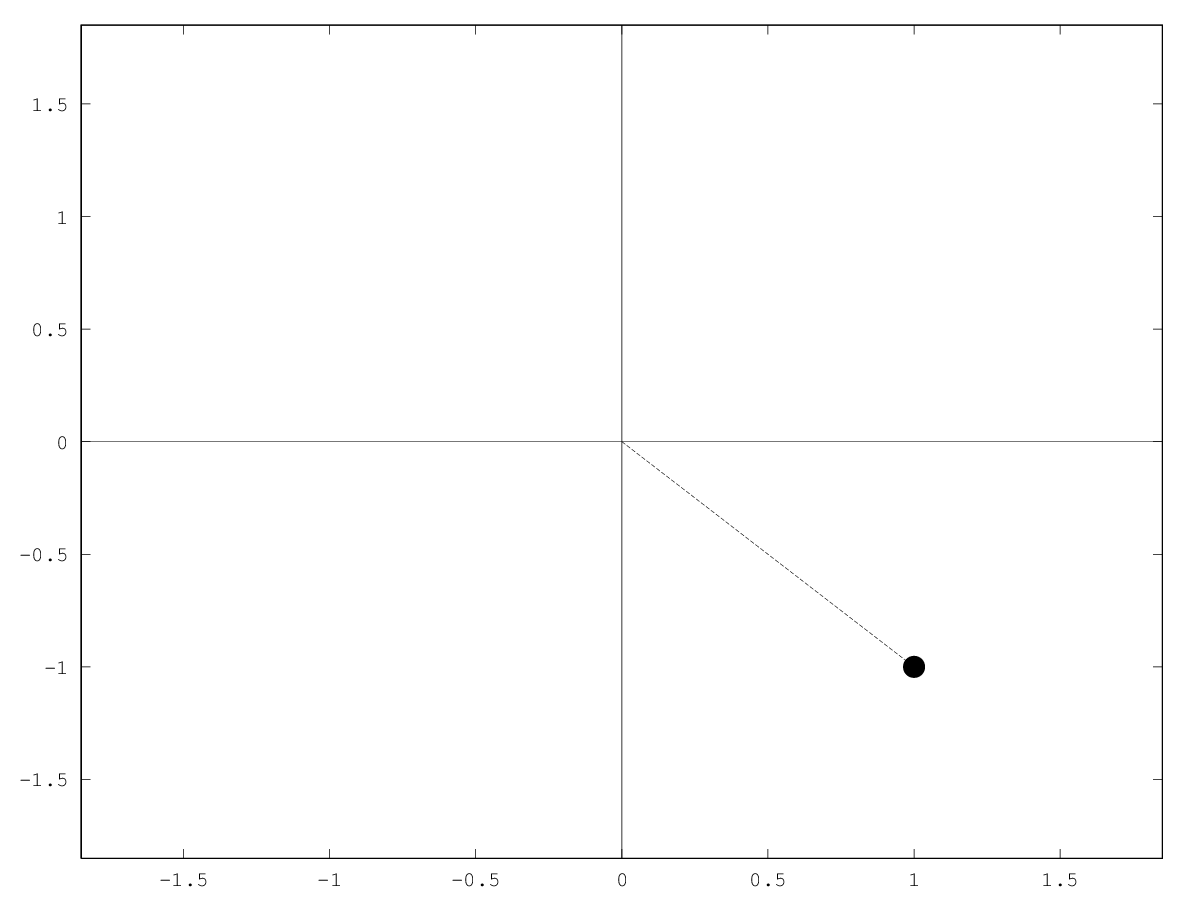
\includegraphics[width=4cm]{img/complexNumber+1-i}}
        
      }

        \vfill
      \item $-1+2i$

      \iftoggle{solutions}{%

        \begin{eqnarray*}
          r & = & \sqrt{(-1)^2 + (2)^2}, \\
            & = & \sqrt{5}, \\
          \tan(\theta) & = & \frac{2}{-1}, \\
          \theta & \approx & 2.03, \\
          z & \approx & \sqrt{5}e^{i2.03}.
        \end{eqnarray*}
        
        \centerline{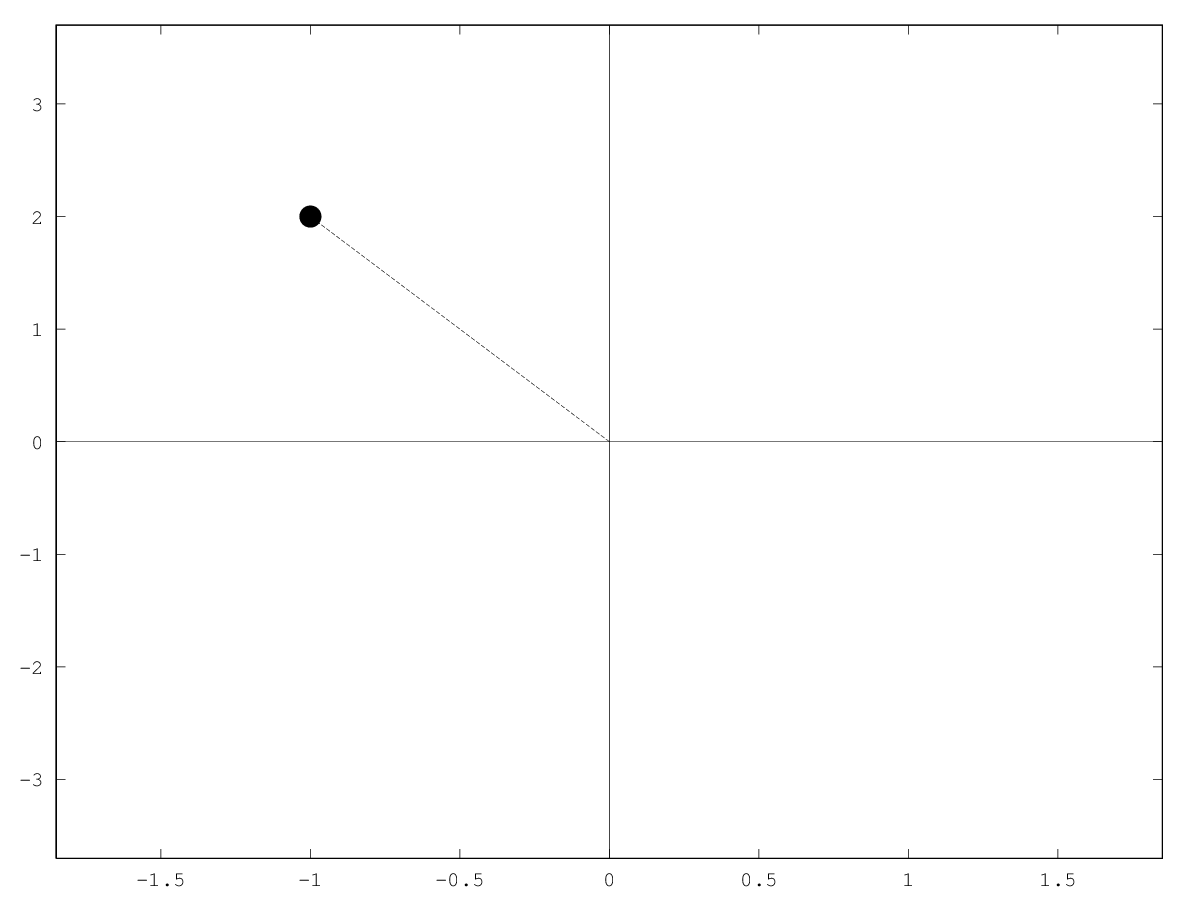
\includegraphics[width=4cm]{img/complexNumber-1+2i}}
        
      }

        \vfill
      \item $-3-i$

      \iftoggle{solutions}{%

        \begin{eqnarray*}
          r & = & \sqrt{(-3)^2 + (-1)^2}, \\
            & = & \sqrt{10}, \\
          \tan(\theta) & = & \frac{-1}{-3}, \\
          \theta & \approx & -2.82, \\
          z & \approx & \sqrt{5}e^{-i2.82}.
        \end{eqnarray*}
        
        \centerline{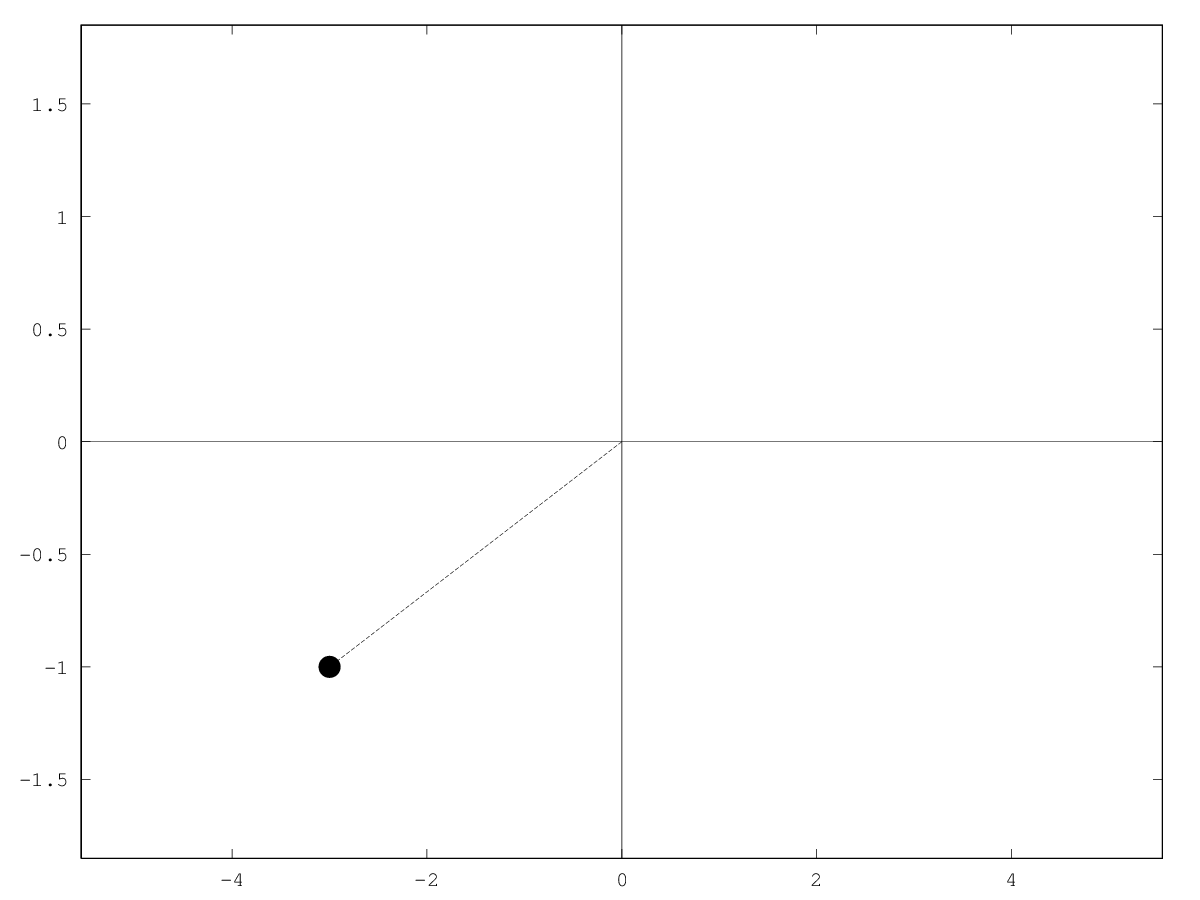
\includegraphics[width=4cm]{img/complexNumber-3-i}}
        
      }

        \vfill
    \end{subproblem}

    \clearpage

  \item Determine the values of the roots. For each problem show the
    graphical representation of the root in relation to the number
    that you are taking the root of.
    \begin{subproblem}
      \item $\sqrt[4]{i}$. 

      \iftoggle{solutions}{%

        \begin{eqnarray*}
          z & = & r e^{i\theta}, \\
          z^4 & = & r^4 e^{i4\theta}, \\
          r^4 e^{i4\theta} & = & e^{i\pi/2},~e^{i5\pi/2},~e^{i9\pi/2},~e^{i13\pi/2}, \\
          z & = & e^{i\pi/8},~e^{i5\pi/8},~e^{i9\pi/8},~e^{i13\pi/8}.
        \end{eqnarray*}
        
      }

        \vfill

      \item $\sqrt[3]{1}$.

      \iftoggle{solutions}{%

        \begin{eqnarray*}
          z & = & r e^{i\theta}, \\
          z^3 & = & r^3 e^{i3\theta}, \\
          r^3 e^{i3\theta} & = & e^{i0},~e^{i2\pi},~e^{i4\pi}, \\
          z & = & 1,~e^{i2\pi/3},~e^{i4\pi/3}.
        \end{eqnarray*}
        
      }

        \vfill

      \item $\sqrt{-4}$.

      \iftoggle{solutions}{%

        \begin{eqnarray*}
          z & = & r e^{i\theta}, \\
          z^2 & = & r^2 e^{i2\theta}, \\
          r^2 e^{i2\theta} & = & e^{i\pi},~e^{i3\pi}, \\
          z & = & e^{i\pi/2},~e^{i3\pi/2}.
        \end{eqnarray*}
        
      }

        \vfill

      \item $\sqrt[5]{1+i}$.

      \iftoggle{solutions}{%

        \begin{eqnarray*}
          z & = & r e^{i\theta}, \\
          z^5 & = & r^5 e^{i5\theta}, \\
          r^5 e^{i5\theta} & = & \sqrt{2}e^{i\pi/4},~\sqrt{2}e^{i9\pi/2},~\sqrt{2}e^{i17\pi/2},~\sqrt{2}e^{i25\pi/2},~\sqrt{2}e^{i33\pi/2}, \\
          z & = & 2^{1/10}e^{i\pi/20},~2^{1/10}e^{i9\pi/20},~2^{1/10}e^{i17\pi/20},~2^{1/10}e^{i25\pi/20},~2^{1/10}e^{i33\pi/20}.
        \end{eqnarray*}
        
      }

        \vfill

    \end{subproblem}

    \clearpage



  \end{problem}
